\documentclass[tikz,border=5pt]{standalone}
\usepackage{ctex}
\usepackage{amsmath,bm}
\usetikzlibrary{arrows.meta,calc}
\definecolor{pb}{RGB}{58,119,168}
\definecolor{oxy}{RGB}{179,68,57}
\definecolor{field}{RGB}{40,105,160}
\definecolor{polar}{RGB}{43,122,90}
\tikzset{arr/.style={-{Stealth[length=2mm]},thick},dim/.style={<->,thin},pb/.style={circle,draw=pb!85!black,fill=pb!28,inner sep=2.7pt},ox/.style={circle,draw=oxy!85!black,fill=oxy!22,inner sep=2.2pt},ti/.style={circle,draw=black,fill=black,inner sep=1.5pt}}
\newcommand{\cell}[2]{%
  \begin{scope}[x={(1.8cm,0cm)},y={(.72cm,.52cm)},z={(0cm,#1cm)}]
  % The rear-bottom-left vertex has three hidden edges.
  \draw[dashed,gray!65] (0,1,0)--(0,0,0) (0,1,0)--(1,1,0) (0,1,0)--(0,1,1);
  \draw[gray!85] (0,0,0)--(1,0,0)--(1,0,1)--(0,0,1)--cycle;
  \draw[gray!85] (1,0,0)--(1,1,0)--(1,1,1)--(1,0,1);
  \draw[gray!85] (0,0,1)--(0,1,1)--(1,1,1);
  \draw[oxy!45,thin] (.5,.5,1)--(.5,1,.5)--(0,.5,.5)--(.5,0,.5)--(1,.5,.5)--(.5,1,.5);
  \draw[oxy!45,thin] (.5,.5,1)--(0,.5,.5) (.5,.5,1)--(.5,0,.5) (.5,.5,1)--(1,.5,.5);
  \draw[oxy!45,dashed,thin] (.5,.5,0)--(.5,1,.5) (.5,.5,0)--(0,.5,.5);
  \draw[oxy!45,thin] (.5,.5,0)--(.5,0,.5) (.5,.5,0)--(1,.5,.5);
  \foreach \xx in {0,1}{\foreach \yy in {0,1}{\foreach \zz in {0,1}{\node[pb] at (\xx,\yy,\zz) {};}}}
  \foreach \p in {(.5,.5,0),(.5,1,.5),(0,.5,.5),(.5,.5,1),(.5,0,.5),(1,.5,.5)}{\node[ox] at \p {};}
  \node[ti] at (.5,.5,#2) {};
  \end{scope}}
\begin{document}
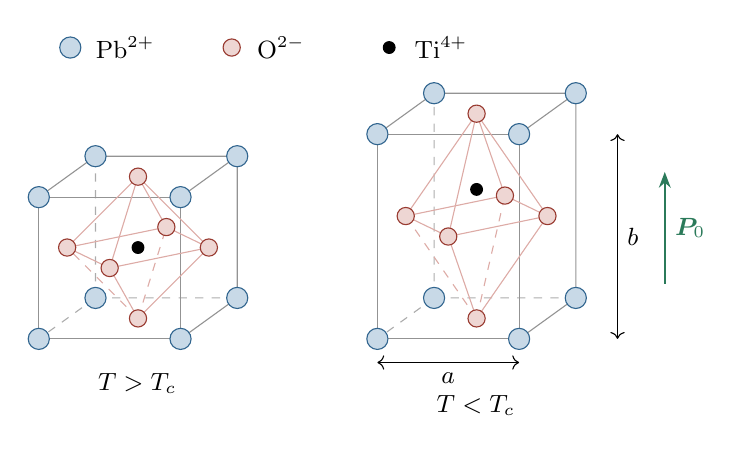
\begin{tikzpicture}[font=\small]
  \begin{scope}\cell{1.8}{.5}\node at (1.25,-.57) {$T>T_c$};\end{scope}
  \begin{scope}[shift={(4.3,0)}]\cell{2.6}{.63}
    \draw[dim] (0,-.3)--(1.8,-.3) node[midway,below] {$a$};
    \draw[dim] (3.05,0)--(3.05,2.60) node[midway,right] {$b$};
    \draw[arr,polar] (3.65,.70)--(3.65,2.12) node[midway,right] {$\bm P_0$};
    \node at (1.25,-.85) {$T<T_c$};
  \end{scope}
  \begin{scope}[shift={(.4,3.70)}]
    \node[pb] at (0,0) {};\node[anchor=west] at (.20,0) {$\mathrm{Pb}^{2+}$};
    \node[ox] at (2.05,0) {};\node[anchor=west] at (2.25,0) {$\mathrm O^{2-}$};
    \node[ti] at (4.05,0) {};\node[anchor=west] at (4.25,0) {$\mathrm{Ti}^{4+}$};
  \end{scope}
\end{tikzpicture}

\begin{tikzpicture}[font=\small]
  \draw[gray!60] (-1.35,-1.5) rectangle (1.35,1.5);
  \draw[dashed,gray] (-1.35,0)--(1.35,0);
  \draw[dashed,gray] (0,-1.5)--(0,1.5);
  \node[ox] at (0,-1.5) {};\node[ox] at (0,1.5) {};
  \node[circle,draw=black,fill=white,inner sep=1.5pt] (O) at (0,0) {};
  \node[below left] at (O) {$O$};
  \node[ti] (I) at (0,.50) {};\node[right=3pt] at (I) {$\mathrm{Ti}^{4+}$};
  \draw[dim] (-.65,0)--(-.65,.50) node[midway,left] {$\delta=\lambda b$};
  \draw[dim] (1.95,-1.5)--(1.95,1.5) node[midway,right] {$b$};
  \draw[arr] (-1.85,-1.4)--(-1.85,1.35) node[above] {$z$};
  \node[below,align=center] at (.10,-1.85) {对称背景的偶极矩为零\\$p_{\mathrm{cell},z}=4e\delta$};
\end{tikzpicture}

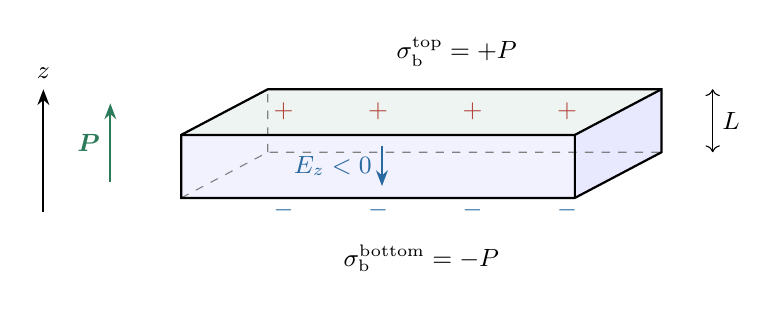
\begin{tikzpicture}[font=\small]
  % A wide plate, not an enlarged unit cell: x and y are in-plane.
  \coordinate (A) at (0,0);\coordinate (B) at (5.0,0);
  \coordinate (C) at (5.0,.80);\coordinate (D) at (0,.80);
  \coordinate (Ap) at (1.10,.58);\coordinate (Bp) at (6.10,.58);
  \coordinate (Cp) at (6.10,1.38);\coordinate (Dp) at (1.10,1.38);
  \fill[blue!5] (A)--(B)--(C)--(D)--cycle;
  \fill[blue!9] (B)--(Bp)--(Cp)--(C)--cycle;
  \fill[polar!8] (D)--(C)--(Cp)--(Dp)--cycle;
  \draw[dashed,gray] (A)--(Ap)--(Bp) (Ap)--(Dp);
  \draw[thick] (A)--(B)--(Bp)--(Cp)--(Dp)--(D)--cycle;
  \draw[thick] (D)--(C)--(Cp) (B)--(C);
  \foreach \xx in {1.3,2.5,3.7,4.9}{\node[oxy] at (\xx,1.10) {$+$};\node[field] at (\xx,-.16) {$-$};}
  \draw[arr,field] (2.55,.66)--(2.55,.15) node[midway,left] {$E_z<0$};
  \draw[arr,polar] (-.90,.20)--(-.90,1.20) node[midway,left] {$\bm P$};
  \draw[dim] (6.75,.58)--(6.75,1.38) node[midway,right] {$L$};
  \draw[arr] (-1.75,-.18)--(-1.75,1.38) node[above] {$z$};
  \node[above] at (3.5,1.55) {$\sigma_{\mathrm b}^{\mathrm{top}}=+P$};
  \node[below] at (3.05,-.47) {$\sigma_{\mathrm b}^{\mathrm{bottom}}=-P$};
\end{tikzpicture}

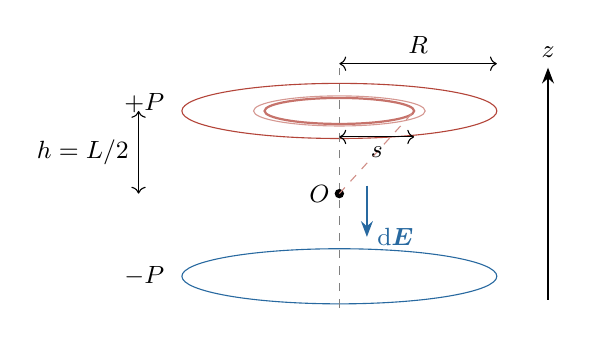
\begin{tikzpicture}[font=\small,arr/.style={-{Stealth[length=2mm]},thick}]
  \draw[oxy] (-2.0,1.05) ellipse (2.0 and .35);
  \draw[field] (-2.0,-1.05) ellipse (2.0 and .35);
  \draw[dashed,gray] (-2,-1.45)--(-2,1.60);
  \fill (-2,0) circle (1.7pt) node[left] {$O$};
  \draw[arr] (.65,-1.35)--(.65,1.60) node[above] {$z$};
  \draw[dim] (-4.55,0)--(-4.55,1.05) node[midway,left] {$h=L/2$};
  \draw[dim] (-2,1.65)--(0,1.65) node[midway,above] {$R$};
  \draw[oxy!75,thick] (-2,1.05) ellipse (.95 and .165);
  \draw[oxy!55] (-2,1.05) ellipse (1.09 and .191);
  \draw[dashed,oxy!60] (-2,0)--(-1.05,1.05);
  \draw[dim] (-2,.72)--(-1.05,.72) node[midway,below] {$s$};
  \draw[arr,field] (-1.65,.10)--(-1.65,-.55) node[right] {$\mathrm d\bm E$};
  \node[left] at (-4.1,1.15) {$+P$};\node[left] at (-4.1,-1.05) {$-P$};
\end{tikzpicture}
\end{document}
